%%%  Ukázkový text a dokumentace stylu pro text závěrečné (bakalářské a
%%%  diplomové) práce na KI PřF UP v Olomouci
%%%  Copyright (C) 2012 Martin Rotter, <rotter.martinos@gmail.com>
%%%  Copyright (C) 2014 Jan Outrata, <jan.outrata@upol.cz>


%%  Pro získání PDF souboru dokumentu je třeba tento zdrojový text v
%%  LaTeXu přeložit (dvakrát) programem pdfLaTeX.

%%  V případě použití programu BibLaTeX pro tvorbu seznamu literatury
%%  je poté ještě třeba spustit program Biber s parametrem jméno
%%  souboru zdrojového textu bez přípony a následně opět (dvakrát)
%%  přeložit zdrojový text programem pdfLaTeX.

%%  Postup získání Postscriptového souboru je popsán v dokumentaci.


%%  Třída dokumentu implementující styl pro závěrečnou práci. Vybrané
%%  nepovinné parametry (ostatní v dokumentaci):

%%  'master' pro sazbu diplomové práce, jinak se sází bakalářská práce

%%  'field=kód' pro Váš studijní obor, kódy pro diplomovou práci 'uvt'
%%  pro Učitelství výpočetní techniky pro střední školy a 'binf' pro
%%  Bioinformatiku, jinak je výchozí Informatika, a pro bakalářskou
%%  práci 'ainfk' pro Aplikovanou informatiku v kombinované formě,
%%  'inf' pro Informatiku, 'infv' pro Informatiku pro vzdělávání a
%%  'binf' pro Bioinfomatiku, jinak je výchozí Aplikovaná informatika
%%  v prezenční formě

%%  'printversion' pro sazbu verze pro tisk (nebarevné logo a odkazy,
%%  odkazy s uvedením adresy za odkazem, ne odkazy do rejstříku),
%%  jinak verze pro prohlížeč

%%  'biblatex' pro zapnutí podpory pro sazbu bibliografie pomocí
%%  BibLaTeXu, jinak je výchozí sazba v prostředí thebibliography

%%  slovak pro slovenský, jinak je výchozí czech pro český

%%  'font=sans' pro bezpatkový font (Iwona Light), jinak výchozí
%%  patkový (Latin Modern)

\documentclass[
%  master,
  field=inf,
%  printversion,
  biblatex,
%  language=english,
%  font=sans,
  glossaries,
  index
]{kidiplom}

%% Informace pro úvodní strany. V jazyku práce (pokud není v komentáři
%% uvedeno česky) a anglicky. Uveďte všechny, u kterých není v
%% komentáři uvedeno, že jsou volitelné. Při neuvedení se použijí
%% výchozí texty. Text pro jiný než nastavený jazyk práce (nepovinným
%% parametrem language makra \documentclass, výchozí český) se zadává
%% použitím makra s uvedením jazyka jako nepovinného parametru.

%% Název práce, česky a anglicky. Měl by se vysázet na jeden řádek.
\title{Grafický editor s výstupem do HTML}
\title[english]{Graphic editor with export to HTML}

%% Volitelný podnázev práce, česky a anglicky. Měl by se vysázet na
%% jeden řádek. Výchozí je prázdný.
\subtitle{}
\subtitle[english]{}

%% Jméno autora práce. Makro nemá nepovinný parametr pro uvedení
%% jazyka.
\author{Zdeněk Mazurák}

%% Jméno vedoucího práce (včetně titulů). Makro nemá nepovinný
%% parametr pro uvedení jazyka.
\supervisor{RNDr. Arnošt Večerka}

%% Volitelný rok odevzdání práce. Výchozí je aktuální (kalendářní)
%% rok. Makro nemá nepovinný parametr pro uvedení jazyka.
%\yearofsubmit{\the\year}

%% Anotace práce, včetně anglické (obvykle překlad z jazyka
%% práce). Jeden odstavec!
\annotation{Cílem této bakalářské práce je vytvoření grafického editoru pro Windows.
Aplikace umožní uživateli kreslit a editovat grafické tvary a text. Všem objektům bude možno nastavit výplň či okraj barvou či gradientem. Editor bude umožňovat export do formátu HTML.}

\annotation[english]{The aim of this bachelor's thesis is to create the graphic editor for Windows. The application will allow the user to draw and edit graphical shapes and text. The user will be able to change the color or gradient of both filling and frame of all present subjects. The editor will allow an exportation to HTML format.}

%% Klíčová slova práce, včetně anglických. Oddělená (obvykle) středníkem.
\keywords{grafický editor; grafické tvary; HTML CANVAS}
\keywords[english]{graphic editor; graphic shapes; HTML CANVAS}

%% Volitelná specifikace příloh textu práce, i anglicky. Výchozí je '1
%% CD/DVD'.
%\supplements{jedno kulaté placaté CD/DVD s malou kulatou dírou uprostřed}
%\supplements[english]{one round flat CD/DVD with a small round hole in the middle}

%% Volitelné poděkování. Stručné! Výchozí je prázdné. Makro nemá
%% nepovinný parametr pro uvedení jazyka.
%%\thanks{Děkuji, děkuji, děkuji.}

%% Cesta k souboru s bibliografií pro její sazbu pomocí BibLaTeXu
%% (zvolenou nepovinným parametrem biblatex makra
%% \documentclass). Použijte pouze při této sazbě, ne při (výchozí)
%% sazbě v prostředí thebibliography.
\bibliography{bibliografie.bib}

%% Další dodatečné styly (balíky) potřebné pro sazbu vlastního textu
%% práce.
\usepackage{lipsum}

\begin{document}
%% Sazba úvodních stran -- titulní, s bibliografickými údaji, s
%% anotací a klíčovými slovy, s poděkováním a prohlášením, s obsahem a
%% se seznamy obrázků, tabulek, vět a zdrojových kódů (pokud jejich
%% sazba není vypnutá).
\maketitle

%% Vlastní text závěrečné práce. Pro povinné závěry, před přílohami,
%% použijte prostředí kiconclusions. Povinná je i příloha s obsahem
%% přiloženého CD/DVD.

%% -------------------------------------------------------------------

\newcommand{\BibLaTeX}{\textsc{Bib}\LaTeX}

\section{Úvod}

Při tvorbě aplikace byl kladen důraz na jednoduché a uživatelsky přívětivé rozhraní. Hlavní inspirace pochází ze známého programu Malování z MS Windows, který je jednoduchý, ale má řadu nevýhod, například nepodporuje průhlednost a hlavně všechno co je jednou nakresleno, už později nelze změnit. Oproti malování náš grafický editor tyto nevýhody nemá. Obsahuje navíc správu vrstev a u grafických objektů kromě barev lze použít i přechody barev (gradienty). Aplikace podporuje dva druhy přechodů: lineární a radiální.

Program není určený pro profesionály, ale pro lidi, kteří si za běžných okolností vystačí pouze s Malováním z MS Windows, ale občas se jim hodí nějaké ty pokročilé funkce. Pro většinu práce s obrázky si vystačíme pouze se základními funkcemi, proto není důležité mít přeplácaný program plný zbytečných funkcí, které nám budou brát na přehlednosti.

Pro obyčejné smrtelníky ve světě grafiky je důležité, aby uživatelské rozhraní bylo jednoduché a přehledné. Toho docílíme, že budeme vycházet z jednoduchých principů kreslení.

\newpage

\section{Uživatelské rozhraní}

Následující kapitola popisuje rozložení prvků v uživatelském rozhraní a jejich funkce.

\subsection{Horní panel}
Horní panel aplikace slouží pro výběr nástroje pro práci. Funguje jako přepínač, současně lze zvolit pouze jeden nástroj. Následně uvedu jednotlivé nástroje.

\begin{itemize}
\item Nástroj pro výběr - slouží pro výběr části obrázku, který lze následně klávesovou zkratkou Ctrl+C zkopírovat do schránky a vložit výřez do jiného programu, nebo jej naklonovat.
\item Nástroj pro výběr grafických objektů - slouží pro označení objektu, který chceme editovat.
\item Úsečka - pro kreslení obyčejné úsečky mezi dvěma body.
\item Polyline - Křivka vytvořená spojením n bodů.
\item Elipsa
\item Obdélník
\item Polygon
\item Kvadratická křivka
\item Text
\item Zpět
\item Vpřed
\item Nástroje pro změnu vlastnosti písma (zobrazí se pouze při editaci textu)
\end{itemize}
\newpage
\begin{figure}
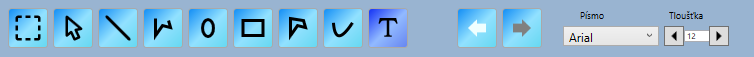
\includegraphics[width=16cm]{img/toppanel}
\caption{Horní panel}
\end{figure}


\subsection{Levý panel}

Horní část levého panelu slouží pro nastavení vlastností grafický objektů. Mezi hlavní vlastnosti patří barvy. V aplikaci můžeme každému objektu nastavit 2 různé barvy: primární a sekundární. Primární slouží u objektů jako barva okraje a sekundární jako barva výplně. Každý objekt však nemá výplň. Například taková úsečka nebo kvadratická křivka výplň nemá a tak na nastavení této vlastnosti nebude reagovat. 

Dále tu máme třetí barvu, která slouží pro nastavení pozadí aktuální vrstvy.

Nastavování těchto těch barev se provádí s pomocí přepínače. Zvolíme jednu z nich a následně jim nastavíme požadovanou barvu. Výběr je možno provést pomocí základních nadefinovaných barev umístěných níže. Pro pokročilejší výběr máme k dispozici paletu barev. Kromě jedné barvy lze nastavit i průhledná nebo přechod více barev.

Na spodní části levého panelu nalezneme správu vrstev. Zde můžeme vrstvy přidávat a nebo mezi nimi přepínat a tak měnit aktivní vrstvu do které aktuálně chceme kreslit. Dále můžeme jednotlivé vrstvy mazat nebo měnit jejich jména či pořadí.

\begin{figure}
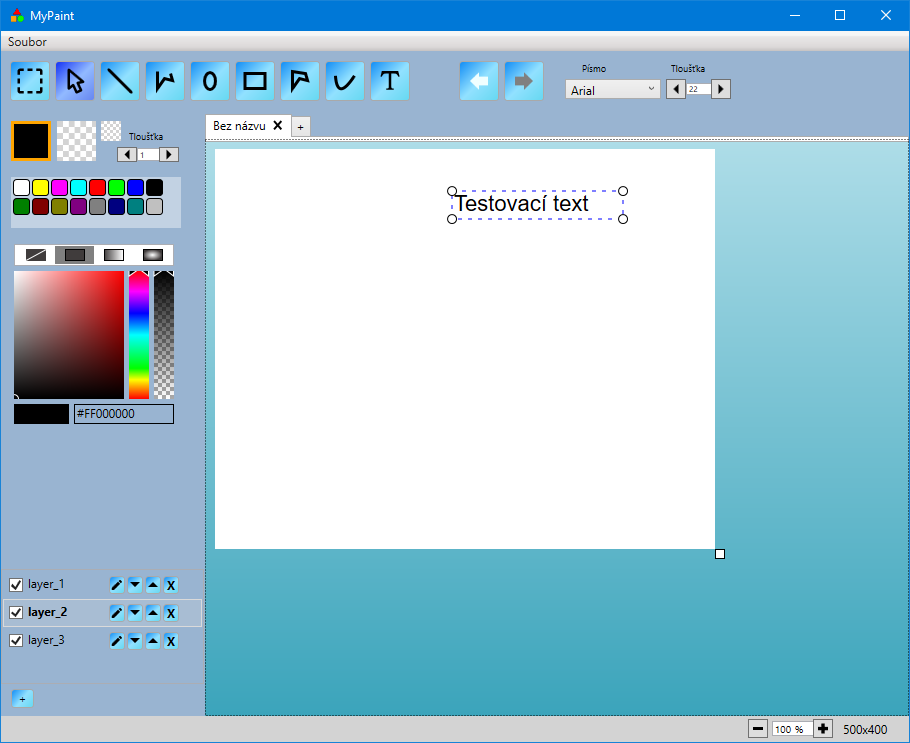
\includegraphics[width=15cm]{img/program}
\caption{Aplikace}
\end{figure}  

\subsection{Kreslící plátno}

Ve středu aplikace se nachází kreslící plátno. Zde můžeme vytvářet a následně upravovat grafické objekty. V pravém dolním rohu kreslícího plátna je umístěn bod pro změnu velkosti plátna. Nad plátnem jsou záložky pro otevřené soubory, program totiž umožňuje upravovat více obrázků najednou.


\section{Funkce}

\subsection{Podporované soubory}

Aplikace podporuje otevírání a ukládání souborů jako rastrovou grafiku ve formátech JPG, PNG a BMP. Při otevření těchto formátů je do plátna načten pouze jeden objekt a tím je celý obrázek. Nelze tak po opětovném otevření upravovat grafické tvary. 

Speciální funkcí této aplikace je ukládání obrázků do formátu HTML. Oproti rastrovým formátům má výhodu v tom, že po otevření jsou načteny do plátna všechny objekty, které je možno dále upravovat. Tento formát reprezentuje obrázek jako vektorovou grafiku. Je možno ho otevřít v jakémkoliv prohlížeči, který podporuje HTML5 Canvas a má zapnutý JavaScript.

\subsection{Uložení do souboru ve formátu HTML}

\subsubsection{HTML soubor}

Soubor s příponou .html nebo .htm je textový soubor, který obsahuje značkovací jazyk HTML. Jazyk se skládá z tagů (značek), které máme párové a nepárové. Do párových tagů můžeme vkládat další HTML tagy nebo text. Vzniká tak v HTML dokumentu stromová struktura. HTML tagy dále obsahují atributy, které mění vlastnosti tagů.

\begin{kicode}{HTML}{kod:HTML}{Ukázka kódu HTML}
<!DOCTYPE html>
<html>
  <head>
  <meta http-equiv="content-type" content="text/html; charset=utf-8">
  <title>Titulek</title>
  </head>
  <body>
    <h1>Nadpis</h1>
    <p>Text</p>
  </body>
</html>
\end{kicode}

\subsubsection{Značka <canvas>}

Formát HTML není určený pro obrázky, ale pro pro webové stránky. Od páté verze HTML podporuje značku <canvas>, která reprezentuje plátno pro kreslení grafiky. Element se umístí do stránky s pevně danou šířkou a výškou. Do plátna pak lze kreslit přes API v JavaScriptu. Pokud změníme jeho rozměry, plátno se vymaže a musíme kreslit znovu.

\begin{kicode}{JavaScript}{kod:JavaScript}{Kreslení obdélníku do canvasu v JavaScriptu}
var c=document.getElementById("myCanvas");
var ctx=c.getContext("2d");
ctx.rect(20,20,150,100);
ctx.stroke();
\end{kicode}

Tahle technologie nám nabízí pomocnou ruku, otázkou je, co uložit do HTML souboru, pokud požadujeme, aby se po otevření souboru ve webovém prohlížeči zobrazil obrázek.

Nabízí se vygenerovat HTML soubor a vložit do něj vygenerovaný program v JavaScriptu, který dokáže obrázek do plátna nakreslit. Tohle řešení by fungovalo, ale mělo by řadu nevýhod. V HTML souboru by bylo spoustu nadbytečného kódu a implementace otevírání HTML souboru, by byla příliš složitá. Nebylo by jednoduché dekódovat program v souboru na grafické objekty. V budoucnu by taky byl problém s kompatibilitou a omezovalo by mě to v případné optimalizaci.

Grafické objekty v aplikaci jsou jen nějaké data uložené v objektech a tak bude jednodušší je tak nechat a zbytečně nepřidávat další balast navíc a to by se přesně stalo, pokud bych se vydal cestou zmíněnou výše. Takže požadujeme tyto objekty uložit do HTML souboru. Protože je HTML soubor textový, musíme tyto objekty reprezentovat pomocí textu. Chceme objekty převést na text a k tomu slouží serializace.

Serializace objektů je proces, který umožňuje objekty programu převést na posloupnost bytů nebo text. Jednoduše umožňuje objekty uložit pro pozdější obnovení.



\subsubsection{JSON}
Aplikace používá serializaci do formátu JSON. JSON je datový formát, který dokáže pojmout datové struktury složených z čísel a řetězců. Často se používá k přenosů dat na internetu, hlavně ve ve webových aplikacích, které využívají technologii AJAX. Další obrovskou výhodou je, že pochází z JavaScriptu. Zkratka JSON totiž znamená \uv{JavaScript Object Notation} což je zápis objektů v JavaScriptu a tak nemusíme programovat žádnou deserializaci, ale postačí nám pouze data v tomto formátu do souboru HTML přiložit.


\subsubsection{Vykreslení obrázku v prohlížeči}
Posledním krokem k zobrazení obrázku v prohlížeči zbývá vykreslit obrázek z přiložených dat v JSONu. Jak už jsem psal výše použijeme k tomu HTML element <canvas>. Do canvasu se kreslí přes API v JavaScriptu, takže získáme přiložená data musíme dostat do programu v JavaScriptu, který bude z dal obrázek vykreslovat do canvasu. 

Data program získá deserializací JSON řetězce. Jelikož je JSON řetězec ekvivalentní se zápisem objektů v JavaScriptu, postačí nám pouze JSON řetězec šikovně uložit k programu.

Program v JS už jen přečte data a vykreslí všechny grafické objekty ve správném pořadí. Pro menší datovou velikost výsledného HTML souboru je kód programu zminifikován. Minifikace nám z kódu odstraní znaky, které nemají vliv na vykonávání kódu. Což jsou pro příklad bílé znaky (mezery, tabulátory, řádky). Dále nahradí názvy promněnných na co nejkratší názvy. Po minifikaci program dělá to stejné jako před ní, jen je o hodně menší. Minifikace je hojně využívaná na internetu a není se čemu divit, všichni přece chceme, aby se internetové stránky načítaly rychle.

\subsubsection{Datová struktura}
Aby byl program v JavaScriptu schopný nakreslit obrázek z přiložených dat, musí mít data určitou datovou strukturu, je velmi podobná struktuře ve kterém aplikace uchovává data při práci s obrázkem.

Všechno začíná třídou Picture, která uchovává rozlišení obrázku a obsahuje vlastnost layers, ve které je uložen seznam vrstev. Jednotlivé vrstvy jsou reprezentovány třídou Layer, která v sobě uchovává barvu pozadí, jméno vrstvy a jestli je vrstva viditelná, jestli se má vykreslit. Mohli by jsme říct, že je zbytečné přikládat vrstvu, která se stejně nenakreslí, ale jelikož jde HTML soubor v aplikaci znovu otevřít a plnohodnotně editovat je dobré ji tam nechat, kdyby s ní ještě chtěl v budoucnu někdo pracovat. To nejdůležitější co třída Layer obsahuje je seznam grafických objektů  umístěný ve vlastnosti shapes.

Grafické objekty jsou reprezentovány třídou Shape. Různé druhy grafických objektů mají hodně odlišné vlastnosti a proto by nebylo moudré všechno ukládat, použijeme tedy dědičnost. Potomky třídy Shape jsou třídy reprezentující jednotlivé druhy grafických objektů, které v sobě uchovávají barvy výplně a okraje, body ze kterých jsou složeny nebo jiné.

Protože serializací objektů do formátu JSON, přijdeme o informaci o informaci z jaké třídy pochází, jelikož JSON formát tyto informace neuchovává. Řešení je jednoduché, stačí přidat všem třídám reprezentují grafické objekty vlastnost type, kde každý druh bude mít unikátní hodnotu. V našem případě je vlastnost type typu řetězec a obsahuje vždy název své třídy. Díky tomu dokáže program jednoduchým způsobem rozpoznat o jaký druh grafického objektu se jedná a podle toho může očekávat vlastnosti.

Zvláštním případem grafického objektu je obrázek, který reprezentuje třída Image a je to obrázek v rastrové grafice. Umožní nám tak ukládat do HTML i rastrovou grafiku. Obrázek je uložen pomocí kódování base64. Base64 je způsob kódování, který kóduje binární data do znaků ASCII.


\begin{figure}
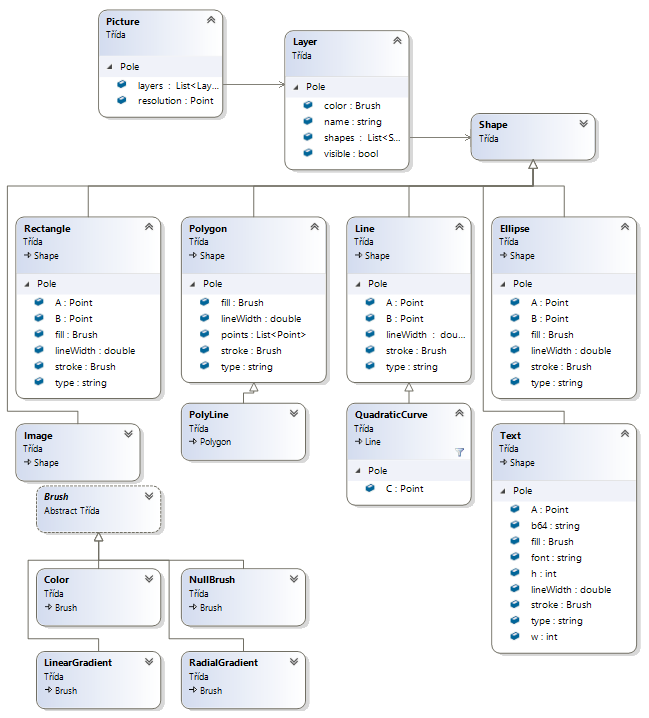
\includegraphics[width=15cm]{img/json_diag}
\caption{Diagram datové struktury pro uložení obrázku do JSONu}
\end{figure} 


\subsection{Uložení do formátů rastrové grafiky}
Aplikace umožňuje uložit obrázky do rastrové (bitmapové) grafiky. Rastrová grafika je způsob ukládání obrázků. Obrázek tímto způsobem je uložen jako barevné body (pixelů, kde každý bod má svojí barvu. Barva pixelů je vyjádřena ve vybraném barevném modelu, v modelu kde můžeme z posloupnosti čísel získat barvu, například model RGB, kde ze třech čísel reprezentující 3 barvy (konkrétně červená, zelená a modrá) dostaneme výslednou barvou jejich smícháním. Existuje i rozšíření modelu RGB, což je model RGBa, kde je navíc ještě čtvrtá složka (alfa kanál), která určuje průhlednost barvy.



\section{Styly pro psaní bakalářských a diplomových prací}
Toto jsou styly pro psaní bakalářských a diplomových prací přes typografický systém \LaTeX{}, tedy \textbf{kistyles}.

\subsection{Požadavky a podprovaná prostředí}
Sada balíku \textbf{kistyles} podporuje následující distribuce systému \LaTeX{}:
\begin{itemize}
\item \TeX{} Live.
\end{itemize}

Jsou podporovány všechny výstupní ovladače, tedy jak \textbf{dvi}, tak \textbf{pdf} i \textbf{ps}. Funkčnost zmiňovaných distribucí byla ověřena na několika operačních systémech, mezi které patří:
\begin{enumerate}
\item Windows $8.1$,
\item Archlinux,
\item Debian.
\end{enumerate}

Důrazně se doporučuje používat aktuální verzi dané distribuce systému \LaTeX{}.

%%%  Po přeložení programem CSLaTeX (třikrát) je potřeba použít
%%%  program DVIPS a takto získaný PostScriptový soubor vytisknout
%%%  na PostScriptové tiskárně nebo pomocí programu GhostScript.
%%%
%%%  Rovněž je možné použít program DVIPDFM a vytvořit z dokumentu
%%%  soubor ve formátu PDF včetně hypertextových odkazů.

\subsection{Přepínače}
Styl kidiplom je z hlediska uživatele zastoupen ekvivalentně nazvanou třídou, kterou je třeba volat na záčátku dokumentu:
\begin{kicode}{TeX}{}{Volání třídy \textbf{kidiplom}}
\documentclass[
  master=true,
  font=sans,
  printversion=false,
  joinlists=true,
  glossaries=true,
  figures=true,
  tables=true,
  sourcecodes=true,
  theorems=true,
  bibencoding=utf8,
  language=czech,
  encoding=utf8,
  field=inf,
  index=true,
  biblatex=true
]{kidiplom}
\end{kicode}

Následuje přehled přepínačů, je vždy uvedeno jméno přepínač, včetně výchozí hodnoty. Přepínače uvádí tabulka \ref{tab:prepinace}.

\begin{table}
\begin{center}
\caption{Seznam přepínačů}\label{tab:prepinace}
\scalebox{0.95}{\begin{tabular}{>{\bfseries}l >{\ttfamily}c L{8cm}}
{\normalfont Přepínač} & {\normalfont Výchozí hodnota} & {\normalfont Popis} \\
\hline
master & false & Povolí nebo zakáže režim diplomové práce. Výchozí režim je tedy bakalářská práce. \\

field & ainfp & Specifikuje studijní obor:\newline
\begin{description}
\item[ainf] Aplikovaná informatika\,--\,prezenční,
\item[ainfk] Aplikovaná informatika\,--\,kombinovaná,
\item[inf] Informatika\,--\,prezenční,
\item[infv] Informatika ve vzdělávání\,--\,kombinovaná,
\item[binf] Bioinformatika\,--\,prezenční.
\end{description} \\

font & serif & Zapne či vypne podporu pěkného bezpatkového fontu. Možné hodnoty jsou:\newline
\begin{description}
\item[sans] Bezpatkové písmo (písmo Iwona).
\item[serif] Patkové písmo (písmo Computer Modern).
\end{description} \\

%%  'encoding=kódování' pro kódování tohoto a vložených zdrojových
%%  textů v kódování jiném než výchozím utf8
encoding & utf8 & Kódování souboru dokumentu, doporučuje se ponechat výchozí hodnotu. \\

bibencoding & utf8 & Kódování souboru bibliografie. Tato volba má smysl pouze, pokud je použita bibliografie skrze balíček \BibLaTeX{}. \\

language & czech & Jazyk práce. \\

printversion & false & Je-li zapnuto, pak budou odkazy vysázeny optimalizovaně pro knižní sazbu. Tuto volbu je nutno použít pro tisk práce. \\

%%% Nepovinné argumenty `tables' a `figures' použijte pouze v případě,
%%% že váš dokument obsahuje tabulky a obrázky a chcete vytvořit
%%% jejich seznamy za obsahem.
%%%
%%% Argument `joinlists' způsobí zřetězení obsahu a seznamů tabulek a obrázků.
%%% Není-li použít, všechny seznamy jsou uvedeny na samostatných stránkách.

joinlists & true & Je-li zapnuto, pak seznamy obrázků, tabulek, vět a
zdrojových kódů sázené za obsahem nebudou rozděleny na samostatné stránky. \\

figures & true & Je-li zapnuto, pak v seznamech položek bude zahrnut seznam obrázků. \\

tables & true & Je-li zapnuto, pak v seznamech položek bude zahrnut seznam tabulek. \\

theorems & false & Je-li zapnuto, pak v seznamech bude zahrnut seznam teorémů. \\

sourcecodes & false & Je-li zapnuto, pak v seznamech bude zahrnut seznam zdrojových kódů. \\

glossaries & false & Je-li zapnuto, pak na konci dokumentu bude vysázen seznam zkratek. \\

index & false & Zapíná podporu sazby rejstříku. \\

biblatex & true & Zapne sazbu bibliografie přes balík \BibLaTeX{}.
\end{tabular}}
\end{center}
\end{table}

\subsection{Geometrie stránky}
Tento styl používá list velikosti $A4$. Pro sazbu prací je třeba použít jednostrannou sazbu. Levý okraj je rozšířen s ohledem na vazbu výsledné knižní podoby práce.

\section{Sazba částí dokumentu}
\subsection{Sazba úvodní strany či obsahu}
Vysázení všech podstatných částí úvodu práce obstará makro \kiinlinecode{TeX}{!}{\\maketitle}. Pro správné vysázení všech částí a meta-informací je potřeba použí makra \kiinlinecode{TeX}{!}{\\title}, \kiinlinecode{TeX}{!}{\\author} a další. Jejich přehled lze najít ve zdrojovém souboru tohoto dokumentu. V případě použítí \textbf{pdf} výstupu se generuje i dodatečná hlavička souboru s meta-informacemi jako je autor dokumentu, název práce či dalšími.

\subsection{Závěry}
Závěr práce by se měl poskytnout jak v původním jazyce práce, tak v jazyce anglickém. Pro sazbu závěru jsou k dispozici příslušná makra. Berte na vědomí, že v anglickém závěru se aktivuje plně anglická sazba se všemi konvencemi. Tedy je třeba používat anglické uvozovky a další správné typografické prvky.

\begin{kicode}{TeX}{}{Sazba závěrů}
% Tiskne český závěr práce.
\begin{kiconclusions}
Závěr práce v \uv{českém} jazyce.
\end{kiconclusions}

% Tiskne anglický závěr práce.
\begin{kiconclusions}[english]
Thesis conclusions written in \uv{English}.
\end{kiconclusions}
\end{kicode}

\subsection{Matematika}
Pro sazbu matematiky je k dispozici sada standardních maker.
$$\langle f \rangle, \lfloor g \rfloor,
\lceil h \rceil, \ulcorner i \urcorner$$

$$\left\{\frac{x^2}{y^3}\right\}$$

$$
A_{m,n} =
 \begin{pmatrix}
  a_{1,1} & a_{1,2} & \cdots & a_{1,n} \\
  a_{2,1} & a_{2,2} & \cdots & a_{2,n} \\
  \vdots  & \vdots  & \ddots & \vdots  \\
  a_{m,1} & a_{m,2} & \cdots & a_{m,n}
 \end{pmatrix}
$$

$$
M = \begin{bmatrix}
       \frac{5}{6} & \frac{1}{6} & 0           \\[0.3em]
       \frac{5}{6} & 0           & \frac{1}{6} \\[0.3em]
       0           & \frac{5}{6} & \frac{1}{6}
     \end{bmatrix}
$$

\subsection{Sazba literatury}
Pro sazbu literatury má uživatel dvě možnosti. Může použít služeb balíků \BibLaTeX{}, který je pro \textbf{kistyles} zapnutý, či lze použít manuální sazbu bibliografie.
\subsubsection{Sazba bibliografie přes \BibLaTeX{}}
Při použití tohoto balíku se data o použité literatuře ukládají do dedikovaného textového souboru, ukázku najdete i v tomto stylu pod jménem \kiinlinecode{text}{!}{bibliografie.bib}.

Formát daného souboru je nad rámec této dokumentace a je na každém uživateli, aby si jej nastudoval. Bibliografie se tiskne makrem \kiinlinecode{TeX}{!}{\\printbibliography}. Taktéž v preambuli dokumentu je třeba definovat, který soubor data bibliografie obsahuje, tedy například \kiinlinecode{TeX}{!}{\\bibliography\{bibliografie.bib\}}.

Dokument, který využívá \BibLaTeX{} je následně nutné přeložit jak pomocí překladače zvoleného ovladače, tak pomocí aplikace \kiinlinecode{text}{!}{biber}. Více informací poskytne soubor \kiinlinecode{text}{!}{Makefile} z distribuce tohoto stylu.

Výhodou tohoto přístupu je, že bibliografie se vysází automaticky a (obvykle) není třeba manuální úprava formátování.

\subsubsection{Manuální sazba bibliografie}
Manuální sazba obnáší vysázení prostředí \kiinlinecode{text}{!}{thebibliography} ručně. To je nad rámec tohoto dokumentu. Ukázku tohoto přístupu lze samozřejmě nalézt ve zdrojovém souboru tohoto dokumentu nebo také \href{http://www.math.uiuc.edu/~hildebr/tex/bibliographies.html}{zde}.

Pro aktivaci manuální sazby bibliografie je třeba volat třídu \kiinlinecode{text}{!}{kidiplom} s parametrem \kiinlinecode{text}{!}{biblatex=false}. Mějte, prosím, na paměti, že v tomto módu jsou makra \kiinlinecode{text}{!}{\\bibliography} a \kiinlinecode{text}{!}{\\printbibliography} nedostupná.

\subsection{Drobná makra}
Základní styl definuje hned několik maker pro usnadnění práce. Například makro \kiinlinecode{TeX}{!}{\\buno} vysází řetezec \uv{bez újmy na obecnosti}. Je k dispozici i verze s prvním velkým písmenem, \kiinlinecode{TeX}{!}{\\Buno}.

Je rovněž možno přidávat položky do seznamu zkratek. K tomu slouží makro \kiinlinecode{TeX}{!}{\\newacronym}, které lze použít například jednoduše jako \kiinlinecode{TeX}{!}{\\newacronym\{UPOL\}\{UPOL\}\{\\kitextunivcz\}}. Na danou zkratku se pak lze odkazovat jednoduše, \kiinlinecode{TeX}{!}{\\gls\{UPOL\}}.

Sazba uvozovek respektuje nastavení částí dokumentu, a proto se doporučuje používat makro \kiinlinecode{TeX}{!}{\\uv}. V anglické závěru práce toto platí taky, viz tato PDF ukázka.

Styl podporuje sazbu odstavců v tabulkách, více obsahuje tabulka \ref{tab:odstavce}.

\begin{table}
\begin{center}
\caption{Seznam přepínačů}\label{tab:odstavce}
\begin{tabular}{L{4cm}|R{4cm}|L{4cm}}
\lipsum[23] & \lipsum[22] & \lipsum[21]
\end{tabular}
\end{center}
\end{table}

K dispozici jsou také makra pro sazbu \csharp{} (\kiinlinecode{TeX}{!}{\\csharp}) či \cpp{} (\kiinlinecode{TeX}{!}{\\cpp}).

%% v případě tvorby rejstříku přeložit vygenerovaný soubor .idx
%% programem Makeindex a v případě tvorby seznamu zkratek spustit
%% program Makeglossaries s parametrem jméno souboru zdrojového textu
%% bez přípony a následně opět (dvakrát) přeložit zdrojový text
%% programem pdfLaTeX.

\subsection{Sazba rejstříku}
Sazba rejstříku sestává z několika kroků:

\begin{enumerate}
\item Je třeba přes volbu \kiinlinecode{TeX}{!}{index=true} rejstříkování povolit.
\item Použítím makra \kiinlinecode{TeX}{!}{\\index} rejstříkovat vybrané pojmy.
\item Kompilovat s použitím utility \kiinlinecode{TeX}{!}{makeindex}. Pro specifika tohoto kroku si stačí prohlédnout soubor \kiinlinecode{text}{!}{Makefile}.
\end{enumerate}

Makro \kiinlinecode{TeX}{!}{\\index} je redefinováno tak, že sází klikací odkaz na výraz v rejstříku. Je doporučeno jej použít ihned za výrazem\index{výraz}.

\textbf{Omezení redefinovaného makra \kiinlinecode{TeX}{!}{\\index}}: klikací odkaz nefunguje, pokud použijete konstrukci \kiinlinecode{TeX}{!}{\\index\{výraz|makro\}} (resp. \kiinlinecode{TeX}{!}{\\index\{výraz|(makro\}}), např. \kiinlinecode{TeX}{!}{\\index\{výraz|textit\}}.

Rejstřík lze vysázet pomocí makra \kiinlinecode{TeX}{!}{\\printindex}.

\subsection{Sazba zdrojových kódů}
Styl nabízí dva způsoby sazby zdrojových kódů:

\begin{enumerate}
\item Sazbu řádkových kódů, například \kiinlinecode{CSS}{!}{background-color: white;}. K tomu slouží makro formátu \kiinlinecode{TeX}{!}{\\kiinlinecode\{jazyk\}\{separátor\}\{kód\}}. Za separátor je vhodné volit jakýkoliv znak, který se nevyskytuje v samotném sázeném zdrojovém kódu. Za jazyk je nutno dosadit jeden z těchto: C, TeX, PHP, HTML, Lisp, SQL, TeX, Python, Java, TutorialD, text, csharp, cpp, JavaScript, CSS.

\item Sazbu zdrojových kódu do separátních prostředí. Takto vytištěný kód se objeví v seznamu zdrojových kódů. Ukázka například zdrojový kód \ref{kod:cpp}. Ukázku sazby naleznete ve zdrojovém kódu tohoto dokumentu.
\end{enumerate}

\newacronym{UPOL}{UPOL}{\kitextunivcz}

\begin{definition}[Název definice]
Abcd. Abcd. Abcd. Abcd. Abcd. Abcd. Abcd. Abcd. Abcd. Abcd. Abcd. Abcd. Abcd. Abcd. Abcd. Abcd. Abcd. Abcd. Abcd. Abcd. Abcd. Abcd. Abcd. Abcd. Abcd. Abcd. Abcd. Abcd. Abcd. Abcd. \gls{UPOL}
\end{definition}

\begin{proof}[Název důkazu]
Abcd. Abcd. Abcd. Abcd. Abcd. Abcd. Abcd. Abcd. Abcd. Abcd. Abcd. Abcd. Abcd. Abcd. Abcd. Abcd. Abcd. Abcd. Abcd. Abcd. Abcd. Abcd. Abcd. Abcd. Abcd. Abcd. Abcd. Abcd. Abcd. Abcd. 
\end{proof}

\begin{remark}[Pumpovací věta]
Abcd. Abcd. Abcd. Abcd. Abcd. Abcd. Abcd. Abcd. Abcd. Abcd. Abcd. Abcd. Abcd. Abcd. Abcd. Abcd. Abcd. Abcd. Abcd. Abcd. Abcd. Abcd. Abcd. Abcd. Abcd. Abcd. Abcd. Abcd. Abcd. Abcd. 
\end{remark}

\begin{example}[Pumpovací věta]
Abcd. Abcd. Abcd. Abcd. Abcd. Abcd. Abcd. Abcd. Abcd. Abcd. Abcd. Abcd. Abcd. Abcd. Abcd. Abcd. Abcd. Abcd. Abcd. Abcd. Abcd. Abcd. Abcd. Abcd. Abcd. Abcd. Abcd. Abcd. Abcd. Abcd. 
\end{example}

\begin{lemma}[Název definice]
Abcd. Abcd. Abcd. Abcd. Abcd. Abcd. Abcd. Abcd. Abcd. Abcd. Abcd. Abcd. Abcd. Abcd. Abcd. Abcd. Abcd. Abcd. Abcd. Abcd. Abcd. Abcd. Abcd. Abcd. Abcd. Abcd. Abcd. Abcd. Abcd. Abcd. 
\end{lemma}

\begin{consequence}[Název důkazu]
Abcd. Abcd. Abcd. Abcd. Abcd. Abcd. Abcd. Abcd. Abcd. Abcd. Abcd. Abcd. Abcd. Abcd. Abcd. Abcd. Abcd. Abcd. Abcd. Abcd. Abcd. Abcd. Abcd. Abcd. Abcd. Abcd. Abcd. Abcd. Abcd. 
\end{consequence}

\begin{theorem}[Pumpovací věta]
Abcd. Abcd. Abcd. Abcd. Abcd. Abcd. Abcd. Abcd. Abcd. Abcd. Abcd. Abcd. Abcd. Abcd. Abcd. Abcd. Abcd. Abcd. Abcd. Abcd. Abcd. Abcd. Abcd. Abcd. Abcd. Abcd. Abcd. Abcd. Abcd. Abcd. 
\end{theorem}


\begin{kicode}{cpp}{kod:cpp}{\cpp}
int main("cs acsa") // komentar
int main("cs acsa") // komentar
int main("cs acsa") // komentar
int main("cs acsa") // komentar
int main("cs acsa") // komentar
\end{kicode}

\begin{kicode}{JavaScript}{}{JS}
new object() // komentar
\end{kicode}

\begin{kicode}{csharp}{}{\csharp}
public static int main("cs acsa") // komentar
\end{kicode}

\begin{kicode}{SQL}{}{SQL}
SELECT * FROM table_1; /* komentar */
\end{kicode}

\begin{kicode}{TutorialD}{}{TutorialD}
table_1 AND table_2;
\end{kicode}

%% Závěry práce. V jazyce práce a anglicky. Text pro jiný než
%% nastavený jazyk práce (nepovinným parametrem language makra
%% \documentclass, výchozí český) se zadává použitím makra s uvedením
%% jazyka jako nepovinného parametru.
\begin{kiconclusions}
Závěr práce v \uv{českém} jazyce.
\end{kiconclusions}

\begin{kiconclusions}[english]
Thesis conclusions in \uv{English}.
\end{kiconclusions}

%% Přílohy obsahu textu práce, za makrem \appendix.
\appendix

\section{První příloha}
Text první přílohy

\section{Druhá příloha}
Text druhé přílohy

%% Obsah přiloženého CD/DVD. Poslední příloha. Upravte podle vlastní
%% práce!
\section{Obsah přiloženého CD/DVD} \label{sec:ObsahCD}

Na samotném konci textu práce je uveden stručný popis obsahu
přiloženého CD/DVD, tj.~jeho závazné adresářové struktury, důležitých
souborů apod.

\begin{description}

\item[\texttt{bin/}] \hfill \\
  Instalátor \textsc{Instalator} programu, popř.~program
  \textsc{Program}, spustitelné přímo z~CD/DVD. / Kompletní adresářová
  struktura webové aplikace \textsc{Webovka} (v~ZIP archivu) pro
  zkopírování na webový server. Adresář obsahuje i~všechny runtime
  knihovny a~další soubory potřebné pro bezproblémový běh instalátoru
  a~programu z~CD/DVD / pro bezproblémový provoz webové aplikace na
  webovém serveru.

\item[\texttt{doc/}] \hfill \\
  Text práce ve formátu PDF, vytvořený s~použitím závazného stylu KI
  PřF UP v~Olomouci pro závěrečné práce, včetně všech příloh,
  a~všechny soubory potřebné pro bezproblémové vygenerování PDF
  dokumentu textu (v~ZIP archivu), tj.~zdrojový text textu, vložené
  obrázky, apod.

\item[\texttt{src/}] \hfill \\
  Kompletní zdrojové texty programu \textsc{Program} / webové aplikace
  \textsc{Webovka} se všemi potřebnými (příp.~převzatými) zdrojovými
  texty, knihovnami a~dalšími soubory potřebnými pro bezproblémové
  vytvoření spustitelných verzí programu / adresářové struktury pro
  zkopírování na webový server.

\item[\texttt{readme.txt}] \hfill \\
  Instrukce pro instalaci a~spuštění programu \textsc{Program}, včetně
  všech požadavků pro jeho bezproblémový provoz. / Instrukce pro
  nasazení webové aplikace \textsc{Webovka} na webový server, včetně
  všech požadavků pro její bezproblémový provoz, a~webová adresa, na
  které je aplikace nasazena pro účel testování při tvorbě posudků
  práce a~pro účel obhajoby práce.

\end{description}

Navíc CD/DVD obsahuje:

\begin{description}

\item[\texttt{data/}] \hfill \\
  Ukázková a~testovací data použitá v~práci a~pro potřeby testování
  práce při tvorbě posudků a~obhajoby práce.

\item[\texttt{install/}] \hfill \\
  Instalátory aplikací, runtime knihoven a~jiných souborů potřebných
  pro provoz programu \textsc{Program} / webové aplikace
  \textsc{Webovka}, které nejsou standardní součástí operačního
  systému určeného pro běh programu / provoz webové aplikace.

\item[\texttt{literature/}] \hfill \\
  Vybrané položky bibliografie, příp.~jiná užitečná literatura
  vztahující se k~práci.

\end{description}

U~veškerých cizích převzatých materiálů obsažených na CD/DVD jejich
zahrnutí dovolují podmínky pro jejich šíření nebo přiložený souhlas
držitele copyrightu. Pro všechny použité (a~citované) materiály,
u~kterých toto není splněno a~nejsou tak obsaženy na CD/DVD, je uveden
jejich zdroj (např.~webová adresa) v~bibliografii nebo textu práce
nebo v souboru \texttt{readme.txt}.

%% -------------------------------------------------------------------

%% Sazba volitelného seznamu zkratek, za přílohami.
\printglossary

%% Sazba povinné bibliografie, za přílohami (případně i za seznamem
%% zkratek). Při použití BibLaTeXu použijte makro
%% \printbibliography. jinak prostředí thebibliography. Ne obojí!

%% Sazba i v textu necitovaných zdrojů, při použití
%% BibLaTeXu. Volitelné.
\nocite{*}
%% Vlastní sazba bibliografie při použití BibLaTeXu.
\printbibliography

%% Bibliografie, včetně sazby, při nepoužití BibLaTeXu.
% \begin{thebibliography}{9}
%\bibitem{kniha2} \uppercase{Hawke}, Paul. NanoHttpd: Light-weight HTTP server designed for embedding in other applications. GitHub [online]. 2014-05-12. [cit. 2014-12-06]. Dostupné z: \url{https://github.com/NanoHttpd/nanohttpd}
%
%\bibitem{jeske13} \uppercase{Jeske}, David; \uppercase{Novák}, Josef. Simple HTTP Server in \csharp: Threaded synchronous HTTP Server abstract class, to respond to HTTP requests. CodeProject: For those who code [online]. 2014-05-24. [cit. 2014-12-06]. Dostupné z: \url{http://www.codeproject.com/Articles/137979/Simple-HTTP-Server-in-C}
%
%\bibitem{uzis2012} \uppercase{ÚSTAV ZDRAVOTNICKÝCH INFORMACÍ A STATISTIKY ČR}. Lékaři, zubní lékaři a farmaceuti 2012 [online]. Praha 2, Palackého náměstí 4: Ústav zdravotnických informací a statistiky ČR, 2012 [cit. 2014-12-06]. ISBN 978-80-7472-089-5. Dostupné z: \url{http://www.uzis.cz/publikace/lekari-zubni-lekari-farmaceuti-2012}
% \end{thebibliography}

%% Sazba volitelného rejstříku, za bibliografií.
\printindex

\end{document}
